% !TeX spellcheck = en_GB
% !TeX program = lualatex
%
% v 2.3  Feb 2019   Volker RW Schaa
%		# changes in the collaboration therefore updated file "jacow-collaboration.tex"
%		# all References with DOIs have their period/full stop before the DOI (after pp. or year)
%		# in the author/affiliation block all ZIP codes in square brackets removed as it was not %         understood as optional parameter and ZIP codes had bin put in brackets
%       # References to the current IPAC are changed to "IPAC'19, Melbourne, Australia"
%       # font for ‘url’ style changed to ‘newtxtt’ as it is easier to distinguish "O" and "0"
%
\documentclass[a4paper,
               %boxit,        % check whether paper is inside correct margins
               %titlepage,    % separate title page
               %refpage       % separate references
               %biblatex,     % biblatex is used
               keeplastbox,   % flushend option: not to un-indent last line in References
               %nospread,     % flushend option: do not fill with whitespace to balance columns
               %hyphens,      % allow \url to hyphenate at "-" (hyphens)
               %xetex,        % use XeLaTeX to process the file
               %luatex,       % use LuaLaTeX to process the file
               ]{jacow}
%
% ONLY FOR \footnote in table/tabular
%
\usepackage{pdfpages,multirow,ragged2e} %
\usepackage{physics}
%
% CHANGE SEQUENCE OF GRAPHICS EXTENSION TO BE EMBEDDED
% ----------------------------------------------------
% test for XeTeX where the sequence is by default eps-> pdf, jpg, png, pdf, ...
%    and the JACoW template provides JACpic2v3.eps and JACpic2v3.jpg which
%    might generates errors, therefore PNG and JPG first
%
\makeatletter%
	\ifboolexpr{bool{xetex}}
	 {\renewcommand{\Gin@extensions}{.pdf,%
	                    .png,.jpg,.bmp,.pict,.tif,.psd,.mac,.sga,.tga,.gif,%
	                    .eps,.ps,%
	                    }}{}
\makeatother

% CHECK FOR XeTeX/LuaTeX BEFORE DEFINING AN INPUT ENCODING
% --------------------------------------------------------
%   utf8  is default for XeTeX/LuaTeX
%   utf8  in LaTeX only realises a small portion of codes
%
\ifboolexpr{bool{xetex} or bool{luatex}} % test for XeTeX/LuaTeX
 {}                                      % input encoding is utf8 by default
 {\usepackage[utf8]{inputenc}}           % switch to utf8

\usepackage[USenglish]{babel}

%
% if BibLaTeX is used
%
\ifboolexpr{bool{jacowbiblatex}}%
 {%
  \addbibresource{jacow-test.bib}
  \addbibresource{biblatex-examples.bib}
 }{}
\listfiles

%%
%%   Lengths for the spaces in the title
%%   \setlength\titleblockstartskip{..}  %before title, default 3pt
%%   \setlength\titleblockmiddleskip{..} %between title + author, default 1em
%%   \setlength\titleblockendskip{..}    %afterauthor, default 1em

\begin{document}

\title{Dual-purpose structure for light and heavy particles}

\author{S. Kolokolchikov\textsuperscript{1,2}, Y. Senichev\textsuperscript{1,2}, A. Aksentyev\textsuperscript{1,2,3}, A. Melnikov\textsuperscript{1,2,4} \\
\textsuperscript{1}Institute for Nuclear Research of the Russian Academy of Sciences, Moscow, Russia\\
\textsuperscript{2}Moscow Institute of Physics and Technology, Dolgoprudny, Russia\\
\textsuperscript{3}National Research Nuclear University MEPhI, Moscow, Russia\\
\textsuperscript{4}Landau Institute for Theoretical Physics, Chernogolovka, Russia\\}
	
\maketitle

%
\begin{abstract}

	\par A dual-purpose structure has been developed for the NICA collider accelerating heavy multiply charged ions and light polarized nuclei of protons and deuterons. For heavy multiply charged ions, it is necessary to solve the problem of intra-beam scattering, which requires minimal modulation of the beta and dispersion function. For light particles, the problem of crossing transition energy arises. In the proposed structure, both problems are solved due to a specially developed structure of magnetic arcs. This lattice can be used to accelerate both heavy ions and light polarized protons and deuterons without a loss of beam quality.

\end{abstract}

\section{Light particle mode}

	In a classical regular lattice, the transition energy is approximately equal to the horizontal betatron tune $\gamma_{\text{tr}}\simeq\nu_{x}$ \cite{b1}. For the same magnetic rigidity $B\rho$, the maximum energy for light particles is greater than for heavy ions due to charge-to-mass ratio. This means heavy ion lattice optimized for operating up to a certain transition energy and would require overcoming for light particle. In general, the transition energy is determined by the momentum compaction factor
\begin{equation}
	\alpha=\frac{1}{{\gamma_{\text{tr}}}^2}=\frac{1}{C}\int_{0}^{C}{\frac{D\left(s\right)}{\rho\left(s\right)}ds},
\end{equation}
	\noindent where $C$ -- orbit length, $D(s)$ -- dispersion function, $\rho(s)$ -- radius of orbit curvature, $s$ -- longitudinal coordinate. It is a characteristic of the lattice and remains constant regardless of the particle type. In the first order the slip-factor $\eta=\eta_0=1/\gamma_{\text{tr}}^2-1/\gamma^2$, and thus the frequency of synchrotron oscillations $\omega_{\text{s}}\ \sim \eta$ tends to zero when the beam energy approaches the transition value. In this case, the adiabaticity of the longitudinal phase motion is violated, which leads to instabilities, as well as the influence of non-linear effects of momentum spread $\delta$. The introduction of modulation into the $D\left(s\right)$ or $\rho\left(s\right)$ function leads to variations in the momentum compaction factor.
\subsection{Resonant Lattice}
The equation for the dispersion function with biperiodic variable focusing \cite{b2}	   
\begin{equation}
	\dv[2]{D}{s}+\left[K(s)+\varepsilon k(s)\right]D=\frac{1}{\rho(s)},
	\label{eq:disp_eq}
\end{equation}
	\noindent where $K\left(s\right)=\frac{e}{p}G\left(s\right)$, $\varepsilon k\left(s\right)=\frac{e}{p}\Delta G\left(s\right)$, $G\left(s\right)$ -- gradient of magneto-optical lenses, $\Delta G\left(s\right)$ -- superperiodic gradient modulation. Here is considered an additional perturbation to regular one $\varepsilon k\left(\phi\right)=\sum_{k=0}^{\infty}g_k\cos(k\phi)$, where $g_k$ -- $k$-th harmonic of the gradient modulation in the Fourier series expansion of the function. The solution for MCF for one superperiod as follows for only gradient modulation
	\begin{equation}
	\begin{aligned}
		\alpha_{\text{s}}= & \frac{1}{\nu^2}\left\{1+\frac{1}{4(1-k S / \nu)}\left(\frac{\bar{R}}{\nu}\right)^4 \frac{g_k^2}{\left[1-(1-k S / \nu)^2\right]^2}\right\},
	\end{aligned}
	\label{eq:alpha_gradient}
	\end{equation}
	\noindent where ${\overline{R}}_{\text{arc}}$ -- the average value of the curvature, $\nu$ -- horizontal betatron tune on arc, $S$ -- number of superperiods per arc. Eq. (\ref{eq:alpha_gradient}) considered without curvature modulation due to the possibility of introducing a transition energy variation into a stationary lattice. For this reason, the sum sign must be negative, this is realizable under the condition $kS/\nu_{x, \text{arc}}>1$.
\begin{figure}[!h]
	\centering
	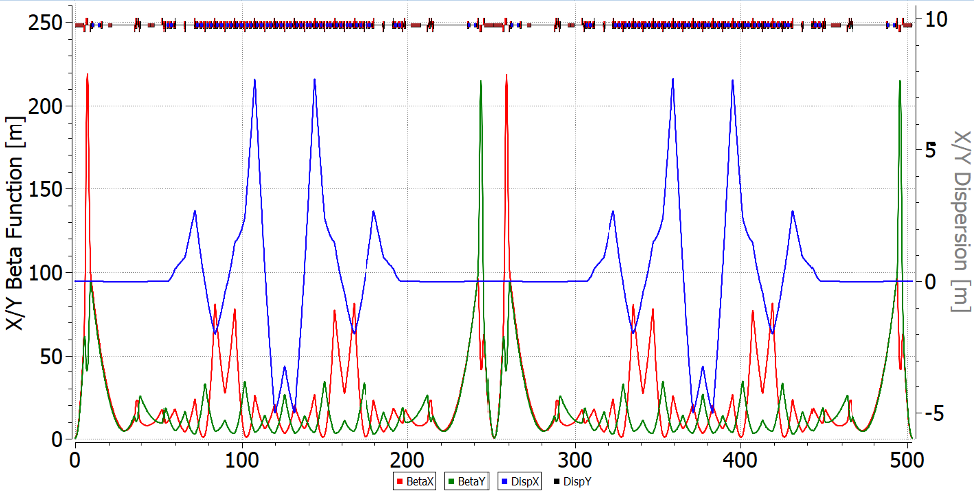
\includegraphics[width=0.9\hsize]{img/MOPM071_f1}
	\caption{Resonant lattice with missing magnet and increased transition energy.}
	\label{fig:resonant}
\end{figure}
	\par First harmonic $k=1$ has a dominant influence, the condition is implemented for $S=4, \nu_{x, \text{arc}}=3$. For a 12 FODO cells per arc, 3 FODO cells are combined into one superperiod \cite{b3}. Thus, an integer number of betatron oscillations on arc, so the arc has first-order achromat property. Straight sections can correct tune for a whole ring to avoid any betatron resonances. Moreover, by according choosing the ratio of superperiod and tune for arc, it is possible to achieve second-order achromat property. Such structure have been considered first for KAON factory \cite{kaon}, later for neutrino factory \cite{neutrino} and implemented at J-PARC \cite{jparc}. It can be also adapt for a lattice with the missing magnet technique (Fig. \ref{fig:resonant}), but the dispersion at the arc's edges must be suppressed \cite{b4}.

\section{Heavy ion mode}\label{sec.III}
	\par The lifetime of the beam luminosity in a collider experiment is achieved through the reduction of intra-beam scattering effects, coupled with the application of stochastic and electron beam cooling techniques. This approach is of particular importance when dealing with high-intensity ion beams. The temporal evolution of emittance in the presence of cooling processes is governed by equation
\begin{equation}
		\dv{\varepsilon}{t} =\underbrace{-\frac{1}{\tau_{\text{tr}}} \cdot \varepsilon}_{\text {cooling}}+\underbrace{\left(\dv{\varepsilon}{t}\right)_{\text{IBS}}}_{\text {heating}},
\end{equation}
	\noindent where $\varepsilon$ -- transverse emittance, $\tau_{\text{tr}}$ -- transverse cooling time, $\tau_{\text{long}}$ -- longitudinal cooling time.
	\noindent For time-independent, stationary values, the time derivatives become zero, then
\begin{equation}
		\varepsilon_{\textrm{st}}=\left.\tau_{\textrm{tr}} \cdot\left(\dv{\varepsilon}{t}\right)_{\textrm{IBS}}\right|_{\varepsilon=\varepsilon_{\textrm{st}}}.
\end{equation}
	The benchmark for evaluating the effectiveness of a cooling technique can be determined by comparing the timescales of stochastic or electron cooling processes with the beam lifetime due to IBS over the entire energy spectrum.

\subsection{Stochastic Cooling}
	\par Let's consider stochastic cooling using the approximate theory developed by D.Mohl \cite{b5, b6}. Based on his main findings, the cooling rate can be determined as
\begin{equation}
	\frac{1}{\tau_{\textrm{tr, l}}}=\frac{W}{N}[\underbrace{2 g \cos \theta\left(1-1 / M_{\textrm{pk}}^2\right)}_{\begin{array}{c}
			\text { \small{coherent} } \\
			\text { \small{effect(cooling)} }
	\end{array}}-\underbrace{g^2\left(M_{\textrm{kp}}+U\right)}_{\begin{array}{c}
			\text { \small{incoherent} } \\
			\text { \small{effect(heating)} },
	\end{array}}],
	\label{eq:stochastic_rate}
\end{equation}	
	\noindent where $W=f_{\text{max}}-f_{\text{min}}$ -- system bandwidth, $N$ -- effective number of particles, $g$ -- fraction of observed sample error corrected per turn, $U$ -- the ratio of noise to signal, $M_{\text{pk}}$, $M_{\text{kp}}$ -- mixing factors between pickup-kicker/kicker-pickup. Eq. (\ref{eq:stochastic_rate}) in the absence of noise at $g=g_0={\frac{1-{M_{\text{pk}}}^2}{M_{\text{kp}}}}$ reaches the maximum
\begin{equation}
		\frac{1}{\tau_{\textrm{tr}}}=\frac{W}{N} \frac{\left(1-1 / M_{\textrm{pk}}^2\right)^2}{M_{\textrm{kp}}}.
	\label{eq:cooling_rate}
\end{equation}
	\noindent The mixing coefficients are defined as
\begin{equation}
	\begin{aligned}
		M_{\textrm{pk}} & =\frac{1}{2\left(f_{\max }+f_{\min }\right) \eta_{\textrm{pk}} T_{\textrm{pk}} \frac{\Delta p}{p}}, \\
		M_{\textrm{kp}} & =\frac{1}{2\left(f_{\max }-f_{\min }\right) \eta_{\textrm{kp}} T_{\textrm{kp}} \frac{\Delta p}{p}},
	\end{aligned}
	\label{eq:mixing_coeff}
\end{equation}
	\noindent where $\eta_{\text{pk}}T_{\text{pk}}\delta$, $\eta_{\text{kp}}T_{\text{kp}}\delta$ -- relative particle displacement times (mixing),  $\eta_{\text{pk}}$, $\eta_{\text{kp}}$ -- slip-factor, as a first approximation, $\alpha_{\text{pk}}$, $\alpha_{\text{kp}}$ -- first-order of local momentum compaction factors, $T_{\text{pk}}$, $T_{\text{kp}}$ -- the absolute times between pickup-kicker/kicker-pickup.

	\par The maximum value of the frequency band is determined by the requirement that the Schottky beam bands do not overlap. In the simplest case, this can be expressed $f_{\textrm{max}}<\frac{1}{\eta_{\textrm{pk}}T_{\textrm{pk}}\frac{\Delta p}{p}}$, thus, a mixing factor $M_{\text{pk}}>1$. Otherwise, the cooling efficiency becomes zero. Modern technologies allow the implementation of a $10$ GHz frequency band \cite{b7}.

	As an example, considered the case of NICA with maximal beam form-factor $F_{\text{bunch}}=4$ with $C_{\text{orb}}=503.04$ m, $\sigma_{\text{bunch}}=0.6$ m, $N_{\text{bunch}}=2.2\cdot{10}^9$. For NICA $f_{\text{max}}=4$ GHz and $f_{\text{min}}=2$ GHz. With these parameters, the maximum achievable cooling rate is $1/\tau_{\text{tr}}=1/230$ $\text{s}^{-1}$.

\par Based on Eq. (\ref{eq:mixing_coeff}), it is evident that asymptotic growth may occur in two scenarios:
\begin{enumerate}
	\item slip-factor approaches the value $\eta\rightarrow\frac{1}{2\left(f_{\text{max}}+f_{\text{min}}\right)T_{\text{pk}}\delta}$,  Schottky spectrum becomes continuous and $M_{\text{pk}}\rightarrow1$;
	\item slip-factor approaches zero, mixing between the kicker to the pickup does not occur and $M_{\text{kp}}\rightarrow\infty$.
\end{enumerate}
	\noindent The efficiency of stochastic cooling depends on the properties of the magneto-optical structure. In classical regular lattices, transition energy is acquired through the horizontal frequency $\gamma_{\text{tr}}\approx\nu_x$ and slip-factor can achieve zero. To avoid asymptotic growth, it is necessary to vary the slip-factor which means $\gamma_{\text{tr}}$. This is possible in resonant lattice, where transition energy can be increased or even reach complex value. In more exotic case, can be used combined lattice then $\eta_{\textrm{pk}}=1/\gamma_{\textrm{tr}}^2-1/\gamma^2$ (pickup-kicker) with real transition energy at one arc compensated by $\eta_{\textrm{kp}}=-1/\gamma_{\textrm{tr}}^2-1/\gamma^2$ (kicker-pickup) with complex transition energy at another for the whole ring. Such structure achieves the required ratio of mixing factors for a maximum cooling rate close to ideal \cite{b9}.
	
	\begin{figure}[!htb]
		\centering
		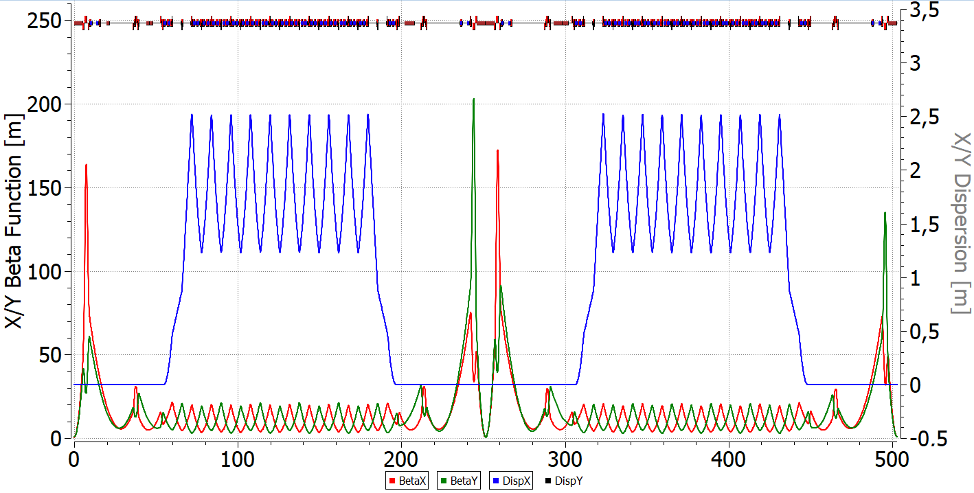
\includegraphics[width=0.9\hsize]{img/MOPM071_f2}
		\caption{Regular lattice with missing magnets.}
		\label{fig:regular}
	\end{figure}
	
	\par The straight sections remains constant in all lattices and essential for analyzing of the resonant characteristics of the entire structure. Their arrangement does not affect the intra-beam scattering and transition energy. To suppress dispersion in the regular lattice, missing magnets technique implemented on both sides of the arc (Fig. \ref{fig:regular}).
	The resonant lattice can be obtained from a regular one by introducing additional family of focusing quadrupoles. To suppress dispersion can be used either two edge focusing quadrupoles on both sides of the arc or only two families of focusing quadrupoles on the arc, when an integer number of betatron oscillations is reached. The combined lattice requires a greater modulation depth of the quadrupoles than in purely resonant lattice with increased transition energy (Fig \ref{fig:combined}).
	
\begin{figure}[!htb]
	\centering
	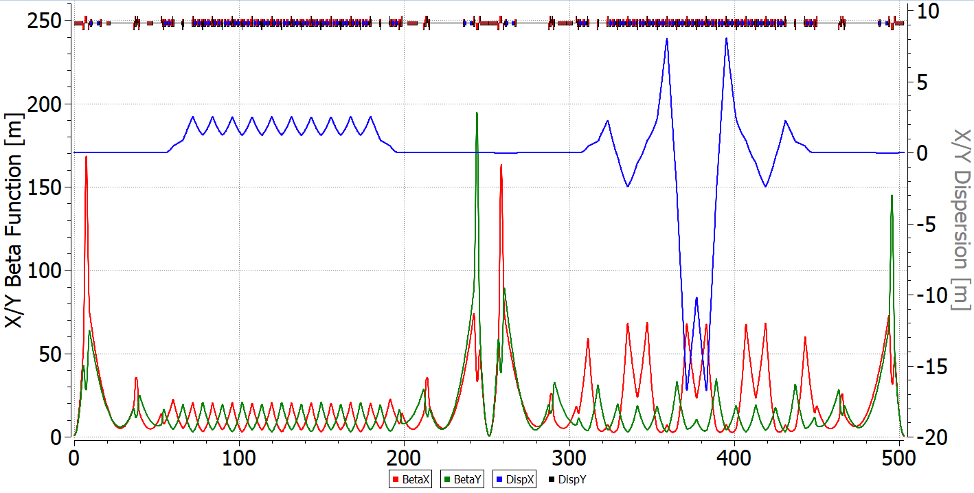
\includegraphics[width=0.9\hsize]{img/MOPM071_f3}
	\caption{Combined lattice with real and complex transition energies in arcs.}
	\label{fig:combined}
\end{figure}	
	
	\noindent As illustrated on Fig. \ref{fig:sc}, for a resonant lattice the second asymptotic is at higher energy compared to regular one. In combined magneto-optics, the cooling efficiency is closer to the ideal in a large energy range $2.5-4.5$ GeV/u, while in regular the cooling rate is almost two times lower at the most optimal point $\sim3$ GeV/u. This behaviour is explained by absence of the second point of asymptotic growth.
	
\begin{figure}[!htb]
	\centering
	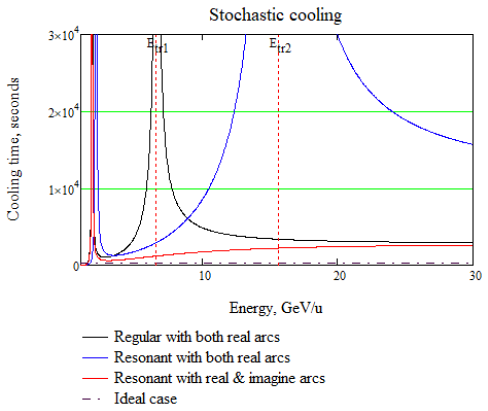
\includegraphics[width=0.9\hsize]{img/MOPM071_f4}
	\caption{The dependence of stochastic cooling time on the energy for various lattices. Energy range 0-30 GeV/u.}
	\label{fig:sc}
\end{figure}

\subsection{Intra-beam Scattering}
\par Intra-beam scattering represents a fundamental limitation on the beam lifetime in the collider. This is derived from the fundamental principles governing this process
\begin{equation}
	\begin{aligned}
		\frac{1}{\tau_{\textrm{IBS}}}=\frac{\sqrt\pi}{4}\frac{cZ^2r_p^2L_C}{A}&\cdot\frac{N}{C_{\mathrm{orb\ }}}\cdot\frac{\left\langle\beta_x\right\rangle}{\beta^3\gamma^3\varepsilon_x^{5/2}\left\langle\sqrt{\beta_x}\right\rangle}\times\\
		&\times\left(\left\langle\frac{D_x^2+{\dot{D}}_x^2}{\beta_x^2}\right\rangle-\frac{1}{\gamma^2}\right)
	\end{aligned}
	\label{eq:ibs}
\end{equation}

\begin{figure}[!htb]
	\centering
	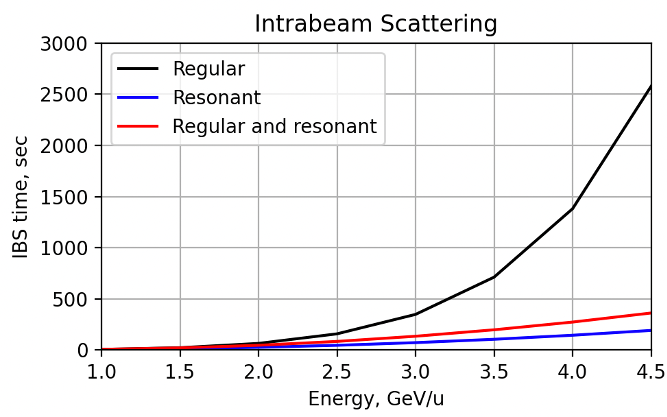
\includegraphics[width=0.8\hsize]{img/MOPM071_f5}
	\caption{The dependence of the beam lifetime due to intra-beam scattering in regular, resonant and combined lattices on the beam energy for heavy ion beam.}
	\label{fig:ibs}
\end{figure}

	\noindent Unlike stochastic cooling, the IBS rate increases as decreasing energy $1/\gamma^3$. In addition, the expression in parentheses is proportional to the slip-factor $\eta$. Therefore, it should be expected that in optics with a value $\eta$ close to zero, the heating rate should decrease. Fig. \ref{fig:ibs} shows the dependences of the heating time constant in the three above-mentioned lattices calculated using MADX programs \cite{b10} for the parameters of the heavy ion beam ${_{79}^{197}}\text{Au}$ of the NICA collider with maximum luminosity ${10}^{27}\ {\text{cm}}^{-2}\text{s}^{-1}$. The corresponding IBS time for heavy and light beam presented at Table \ref{tab:dual} for beam intensities $N_{\text{heavy}} = 2.2\times10^9$ ppb and $N_{\text{light}} = 1\times10^{12}$ ppb with $n_{\text{bunch}}=22$. Consequently, it states that at experiment energy IBS times differ at about 10 times, so the issue of intra-beam scattering becomes critical for heavy-ion beam.
	\par From the comparison of the IBS lifetime with the cooling time it can be concluded that in a regular lattice, stochastic cooling is able to balance intra-beam scattering in the energy range $W\geq4.5\ \text{GeV/u}$. In order to apply stochastic cooling over the entire energy range, it is obvious that we must sacrifice the luminosity of the beam at low energies by increasing the emittance. In resonant lattices, the IBS time is notably reduced. Thus, for the case of heavy ions, the configuration should be regular and minimally modulated. Electron cooling is used lower $4.5$ GeV/u \cite{b11, b12}.

\begin{table}[!htb]
	\caption{Main parameters of lattices.}
	\label{tab:dual}
	\begin{tabular*}{8cm} {lccc}
		\toprule
		Lattice & Regular & Resonant & Combined \\
		\midrule
		Energy, GeV/u & 4.5 & 12.6 & 12.6 \\
		$\gamma_{\text{tr}}$  & 7 & 15 & $i50$ \\
		Modulation depth & -- & 25\% & 45\% \\
	 	$\tau_{\text{SC}}$ for \textbf{Au}, s & 2500 & 1500 & 800 \\
		$\tau_{\text{IBS}}$ for \textbf{Au}, s & 2500 & 400 & 250 \\
		$\tau_{\text{IBS}}$ for \textbf{p}, s & $1.8\times10^{4}$ & $4.5\times10^3$ & $7.9\times10^3$ \\
		\bottomrule
	\end{tabular*}
\end{table}

\section{CONCLUSION}

\par The dual magneto-optical structure is proposed for accelerating both light and heavy particle beams, exemplified by the NICA facility. In a resonant lattice, transition energy can be increased. Regular one is optimal for multiply charged particles due to ratio between IBS and stochastic cooling. To convert a regular lattice into resonant one, it is enough only to introduce a separate family of focusing quadrupoles.

\section{Acknowledgments}

\par A support of thus study by the Russian Science Foundation grant 25-72-30005 is acknowledged.

\ifboolexpr{bool{jacowbiblatex}}
	{\printbibliography}
	{
	\begin{thebibliography}{9}
	
	\bibitem{b1} S.-Y. Lee, {\it Accelerator Physics}, Fourth Edition, World Scientific Publishing Company (Singapore, 2018)
	\bibitem{b2} Y.V. Senichev, A.N. Chechenin, Theory of “Resonant” lattices for synchrotrons with negative momentum compaction factor. J. Exp. Theor. Phys. {\bf 105}, 988–997 (2007). \url{doi:10.1134/S1063776107110118}
	\bibitem{b3} Senichev, Y.V., Chechenin, A.N. Construction of “resonant” magneto-optical lattices with controlled momentum compaction factor. J. Exp. Theor. Phys. {\bf 105}, 1141–1156 (2007). \url{doi:10.1134/S1063776107120060}
	\bibitem{kaon} N.I. Golubeva \emph{at al.}, in {\it Proc. 1991 IEEE Particle Accelerator Conference}, San Francisco, 1991, ed. by Lizama, Loretta and Chew, Joe
	\bibitem{neutrino} B. Autin \emph{at al.}, in {\it Proc. 7th European Conference},  Vienna, 2000, ed. by J.L. Laclare, W. Mitaroff, M. Regler, C. Petit-Jean-Genaz, J. Poole
	\bibitem{jparc}	Y. Mori \emph{at al.}, in {\it Proc. 5th European Conference}, Sitges, 1996, ed. by S. Myers, A. Pacheco, R. Pascual, C. Petit-Jean-Genaz, J. Poole
	\bibitem{b4} S.D. Kolokolchikov, Y.V. Senichev, Magneto-Optical Structure of the NICA Collider with High Transition Energy. Phys. Atom. Nuclei. {\bf 84}, 1734–1742 (2021). \url{doi:10.1134/S1063778821100185}
	\bibitem{b5} D. Möhl, G. Petrucci, L. Thorndahl, S. van der Meer, Physics and technique of stochastic cooling. Phys. Rep. {\bf 58}, 75 (1980). \url{doi:10.1016/0370-1573(80)90140-4}
	\bibitem{b6} D. Möhl, The status of stochastic cooling. Nuc. Inst. and Methods in Phys. Res. {\bf A 391}, 164-171 (1997). \url{doi:10.1016/S0168-9002(97)00360-4}
	\bibitem{b7} F.Caspers, D. Möhl, in {\it Proc. of XVII International Conference High Energy Accelerators}, Dubna, 1998, ed. by I.N. Meshkov
	\bibitem{b9} Yu. Senichev, in {\it Proc. 6th Workshop on Beam Cooling and Related Topics (COOL'07)}, Bad Kreuznach, 2007, ed. by Rainer W. Hasse, Volker R.W. Schaa
	\bibitem{b10} F. Antoniou, F. Zimmermann, Revision of Intrabeam Scattering with Non-Ultrarelativistic Corrections and Vertical Dispersion for MAD-X. (European Organization for Nuclear Research CERN, 2012), \url{https://cds.cern.ch/record/1445924}. Accessed 04 May 2012
	\bibitem{b11} S.A. Kostromin \emph{et al.}, Beam-cooling methods in the NICA project. Phys. Part. Nuclei Lett. {\bf 9}, 322–336 (2012). \url{doi:10.1134/S1547477112040206}
	\bibitem{b12} G. Trubnikov, A. Sidorin, N. Shurkhno, NICA Cooling Programm. Cybern. Phys. {\bf 3}, 137-146 (2014)
	
	\end{thebibliography}
}

\end{document}